\chapter{Temperature Dependence of Electrical Resistance}

\begin{figure}
	\centering
	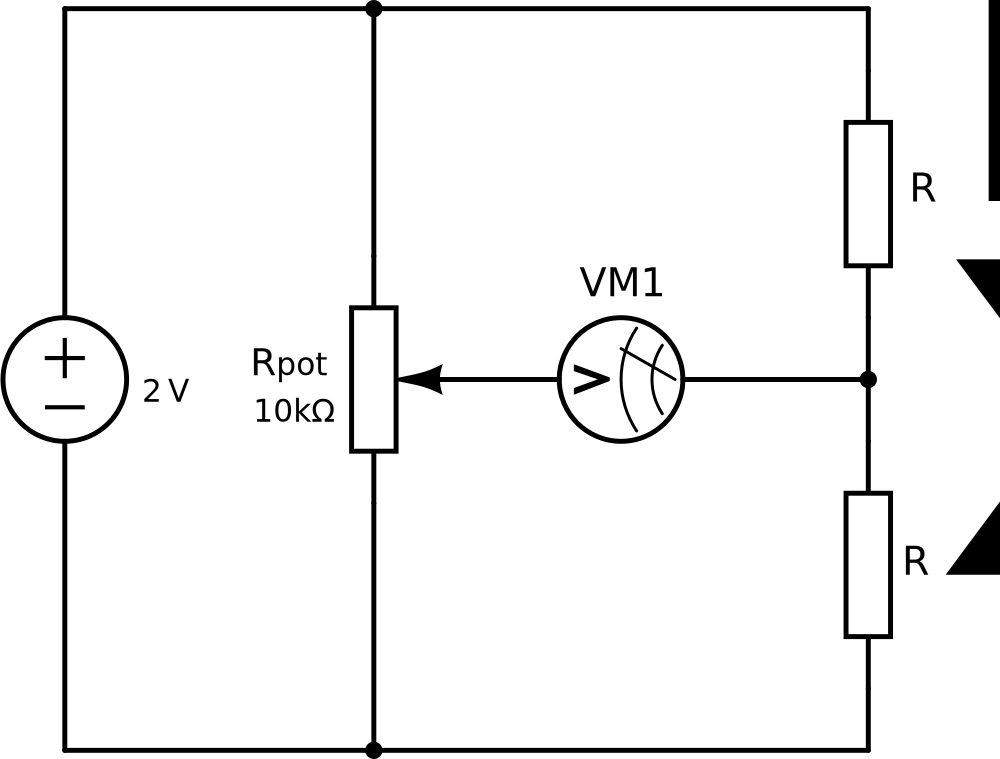
\includegraphics[width=.6\textwidth]{img/sch-wheatstone.pdf}
	\caption{Wheatstone Bridge Schematic}
	\label{sch:wheatstone}
\end{figure}

\begin{figure}
	\centering
	\includegraphics[width=.8\textwidth]{data/plots/tempco.pdf}
	\caption{Temperature Dependence of NTC and PT100}
	\label{plot:tempco}
\end{figure}

The temperature dependence of an NTC and a PT100 thermal sensor are measured.

Temperature is controlled with an oven and is ramped from ambient temperature to \SI{200}{\celsius}.
A digital thermometer is used to monitor the current temperature.

The resistance of the device under test is measured with a Wheatstone bridge (\autoref{sch:wheatstone}).
The voltage differential of the two legs is measured with a digital multimeter.
A multiturn potentiometer fitted with a turn-counting dial is used as one of the legs.

The resistance $R_\text{x}$ of the DUT is calculated as
\begin{alignat}{1}
	\frac{R_\text{set}}{R_\text{pot}} &= \frac{R_\text{x}}{R_\text{x} + R_\text{ref}} \nonumber\\
	\implies R_\text{x} &= R_\text{ref} \; \frac{R_\text{set}}{R_\text{pot} - R_\text{set}},
\end{alignat}
with the resistance of the potentiometer $R_\text{pot}$, it's lower arm $R_\text{set}$ and the reference resistor $R_\text{ref}$.
